\documentclass[tikz,border=10pt]{standalone}

\begin{document}
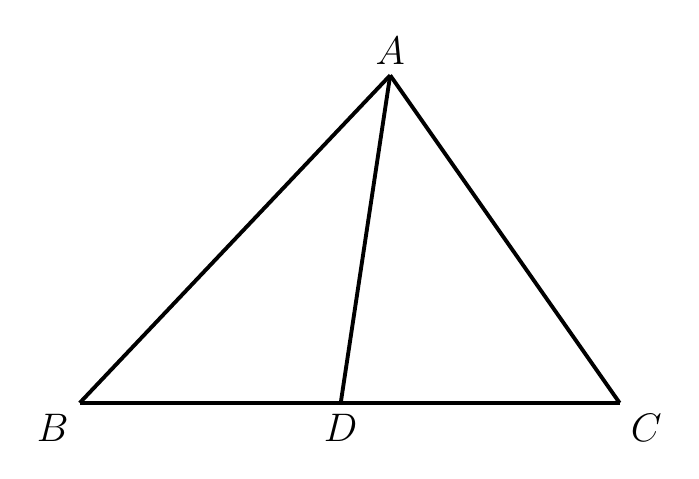
\begin{tikzpicture}[line width=1.4pt, line join=round]
\coordinate (A) at (0.519,2.086);
\coordinate (B) at (-3.424,-2.075);
\coordinate (C) at (3.433,-2.075);
\coordinate (D) at (-0.109,-2.075);

  
  \draw (A) -- (B);
  \draw (A) -- (C);
  \draw (B) -- (C);
  
  \draw (A) -- (D);
  
  \node[above] at (A) {\fontsize{14.5}{17.4}\selectfont $A$};
  \node[below left] at (B) {\fontsize{14.5}{17.4}\selectfont $B$};
  \node[below right] at (C) {\fontsize{14.5}{17.4}\selectfont $C$};
  \node[below] at (D) {\fontsize{14.5}{17.4}\selectfont $D$};
\end{tikzpicture}
\end{document}